\documentclass[11pt,a4paper]{article}

\usepackage[T1]{fontenc}
\usepackage[utf8]{inputenc}
\usepackage{lmodern}
\usepackage[a4paper,margin=2.5cm]{geometry}
\usepackage{graphicx}
\usepackage{float}
\usepackage{caption}
\usepackage{booktabs}
\usepackage{enumitem}
\usepackage[hidelinks]{hyperref}
\usepackage{xurl}

\renewcommand{\figurename}{Slika}
\renewcommand{\tablename}{Tabela}
\renewcommand{\contentsname}{Kazalo}
\renewcommand{\refname}{Viri}
\renewcommand{\listfigurename}{Kazalo slik}

\graphicspath{{slike/}}
\setlength{\emergencystretch}{3em}
\setlist{itemsep=2pt,topsep=4pt}

\begin{document}

\begin{titlepage}
  \centering
  \vspace*{2cm}
  {\large Univerza v Mariboru\\Fakulteta za elektrotehniko, računalništvo in informatiko\par}
  \vspace{3cm}
  {\Huge\bfseries SloFit\par}
  \vspace{0.6cm}
  {\LARGE Pregled obstoječih rešitev\par}
  \vspace{0.4cm}
  {\large Spletna stran za podjetje SloFit\par}
  \vfill
  {\large\bfseries Člani skupine:\par}
  \vspace{0.3cm}
  {\large
    Dino Nuhanović\\
    Mark Kac\\
    Aleksa Kosanović\par}
  \vspace{2cm}
  {\large Maribor, november 2026\par}
\end{titlepage}

\tableofcontents
\newpage

\section{Uvod}

SloFit je slovensko podjetje s sedežem v Mariboru, ki razvija istoimensko mobilno aplikacijo za fitnes in zdrav življenjski slog. Aplikacija je namenjena začetnikom in izkušenim športnikom ter omogoča:
\begin{itemize}
  \item pripravljene načrte vadbe za različne cilje (hujšanje, pridobivanje mišične mase, vzdržljivost),
  \item beleženje opravljenih treningov in napredka,
  \item spremljanje prehrane in vnosa kalorij,
  \item statistiko in grafe napredka,
  \item motivacijske izzive in opomnike.
\end{itemize}
Osnovni del aplikacije je brezplačen, dodatne funkcionalnosti pa so na voljo v plačljivih paketih. Poslanstvo podjetja je ljudem v Sloveniji olajšati pot do bolj zdravega in aktivnega življenja, vizija pa postati najbolj priljubljena slovenska fitnes aplikacija.

V okviru projekta izdelujemo \textbf{spletno stran za podjetje SloFit}. Problem, ki ga rešujemo, je, da mobilna aplikacija sama po sebi nima mesta, kjer bi potencialni uporabnik na enem mestu spoznal njene funkcionalnosti in prednosti, primerjal pakete, aplikacijo prenesel in stopil v stik s podjetjem. Spletna stran bo tako predstavila aplikacijo, njene funkcionalnosti in prednosti ter obiskovalcem omogočila prenos aplikacije in stik s podjetjem.

Da bi ugotovili, kako podobne storitve predstavljajo svoje aplikacije in pakete, smo pregledali štiri uveljavljene rešitve s podobnim poslovnim modelom (brezplačna osnova + plačljiva naročnina): Google Health Premium (prej Fitbit Premium), Strava, Freeletics in Garmin Connect+.


\section{Obstoječe rešitve}

\subsection{Google Health Premium (prej Fitbit Premium)}

\paragraph{Opis.} Fitbit Premium je naročniška storitev za uporabnike naprav Fitbit in Pixel Watch. Maja 2026 je Google storitev preimenoval v \emph{Google Health Premium}, aplikacija Fitbit pa se zdaj imenuje Google Health \cite{freedom251}. Naročnina stane 9,99~USD na mesec oziroma 99,99~USD na leto, kar je 20~USD več od prejšnje letne cene \cite{androidauthority_gh}.

\paragraph{Ključne funkcionalnosti.}
\begin{itemize}
  \item dnevna ocena pripravljenosti (\emph{Daily Readiness Score}), ki združuje napor, spanec in odziv srčnega utripa \cite{wareable_fitbit};
  \item podrobna analiza spanja in stresa;
  \item knjižnica vodenih vadb in meditacij \cite{techradar_fitbit};
  \item osebni trener, ki temelji na umetni inteligenci (Gemini) \cite{googlestore_fitbit}.
\end{itemize}

\paragraph{Prednosti.} Zelo bogata vsebina (vadbe, spanje, prehrana, mentalno zdravje), dober prikaz podatkov s pametne ure, preprosta uporaba.

\paragraph{Slabosti.} Najboljše deluje le z lastnimi napravami (Fitbit, Pixel Watch), cena se je v letu 2026 opazno zvišala, spletna različica za pregled podatkov je skromna -- skoraj vse se dogaja v mobilni aplikaciji.

\begin{figure}[H]
  \centering
  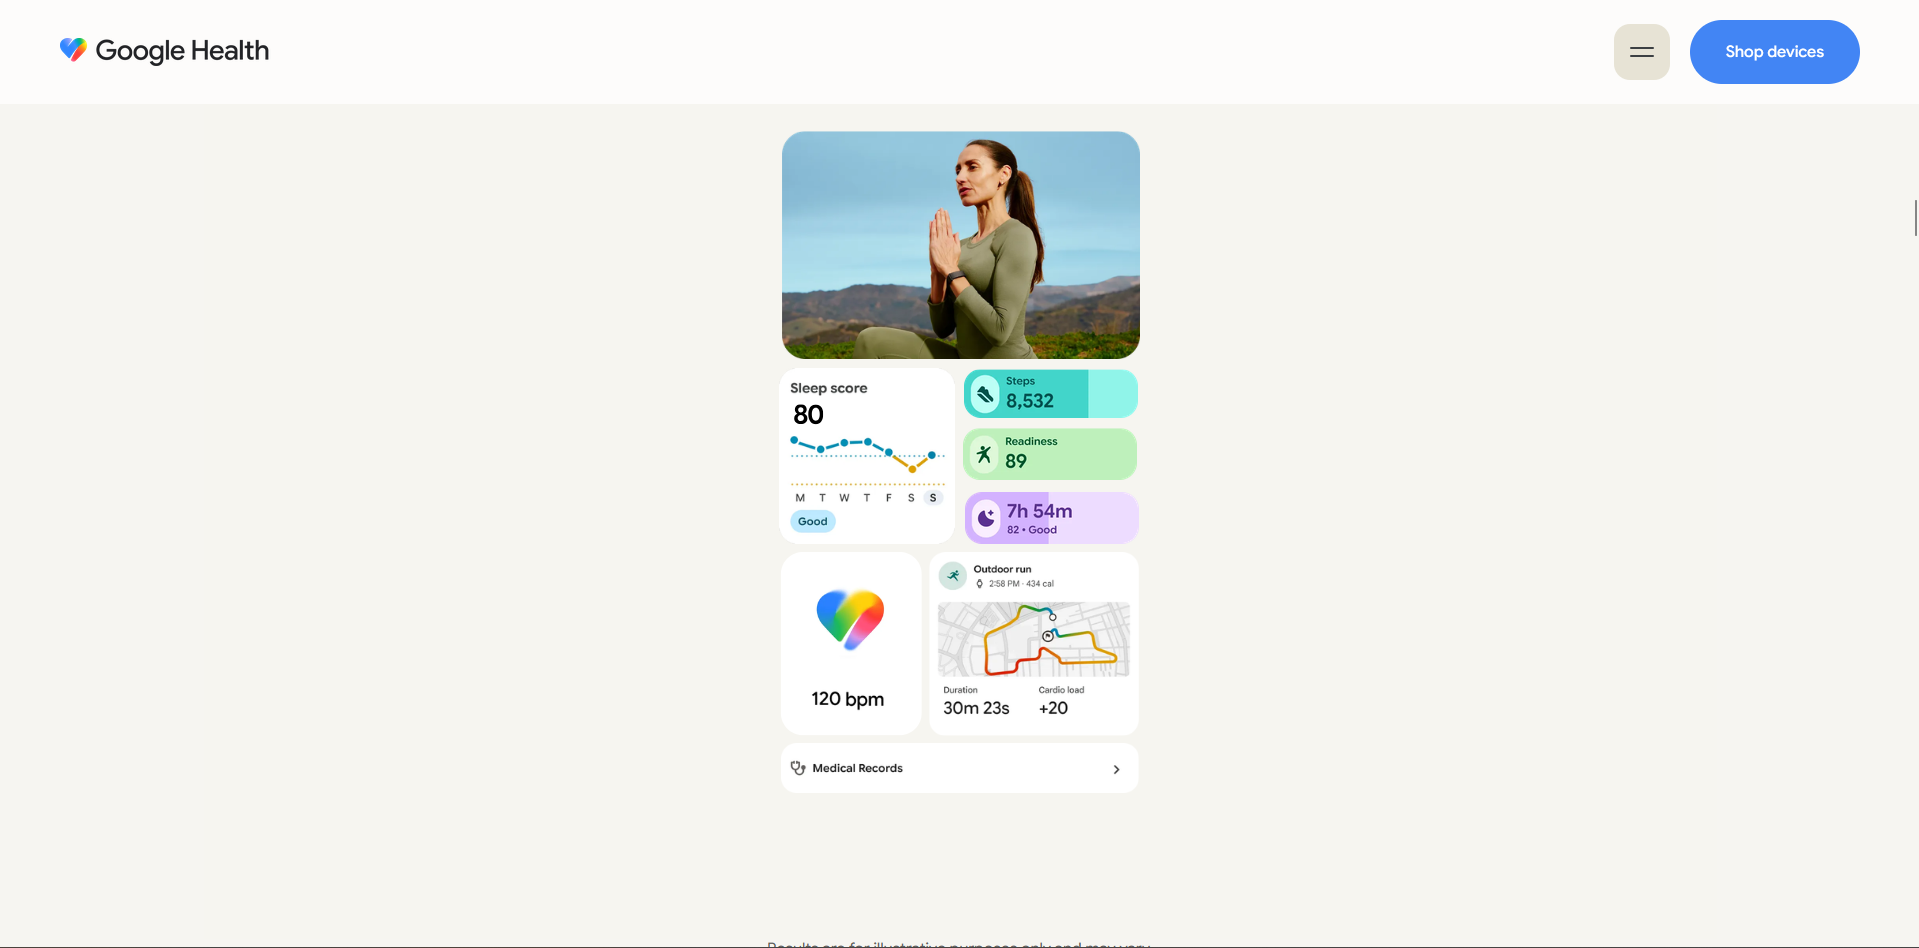
\includegraphics[width=0.85\textwidth]{google_health.png}
  \caption{Spletna stran storitve Google Health Premium \cite{googlestore_fitbit}.}
  \label{fig:google}
\end{figure}

\subsection{Strava}

\paragraph{Opis.} Strava je družbeno omrežje in aplikacija za beleženje teka, kolesarjenja in drugih športov. Osnovna uporaba je brezplačna, naročnina pa odklene napredne funkcije. Cena naročnine se razlikuje glede na državo; v ZDA znaša 11,99~USD na mesec ali 79,99~USD na leto \cite{wareable_strava}.

\paragraph{Ključne funkcionalnosti.}
\begin{itemize}
  \item beleženje aktivnosti z GPS in sinhronizacija z ure (Garmin, Apple, Fitbit \ldots);
  \item načrtovanje poti, lestvice segmentov in nadzorna plošča treninga \cite{bikeradar_strava};
  \item izzivi, klubi in deljenje aktivnosti s prijatelji;
  \item spletna nadzorna plošča z obsežnejšo analizo kot v aplikaciji.
\end{itemize}

\paragraph{Prednosti.} Odlična skupnost in motivacija prek družbenih funkcij, podpora za veliko športov in naprav, enostaven vmesnik \cite{techradar_strava}.

\paragraph{Slabosti.} Nekatere funkcije so na voljo le v spletni različici, cene naročnine so se večkrat zvišale, ne ponuja vodenih vadb za moč ali personaliziranega razporeda vadbe za začetnike \cite{techradar_strava}.

\begin{figure}[H]
  \centering
  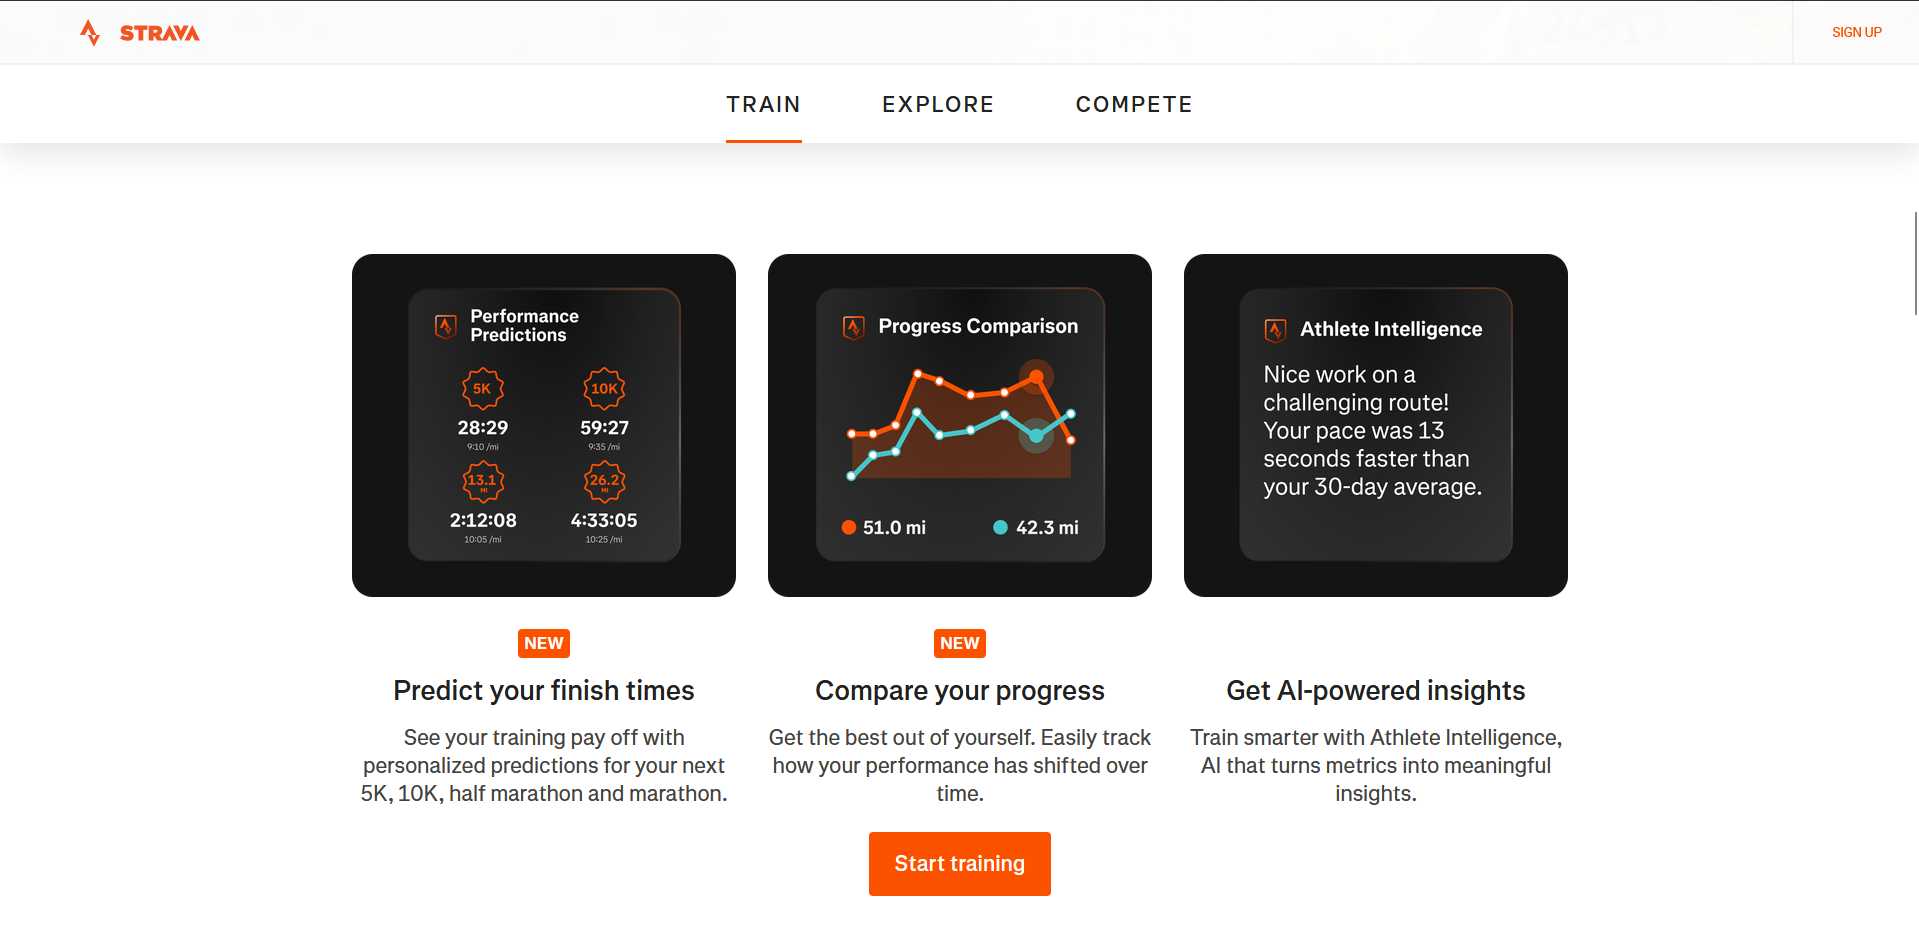
\includegraphics[width=0.85\textwidth]{strava.png}
  \caption{Spletna nadzorna plošča aplikacije Strava \cite{strava_web}.}
  \label{fig:strava}
\end{figure}


\subsection{Freeletics}

\paragraph{Opis.} Freeletics je aplikacija za vadbo z lastno telesno težo (HIIT), ki deluje kot digitalni osebni trener. Brezplačna različica ponuja omejen nabor vadb, plačljivi \emph{Coach} pa ustvari celoten personaliziran program. Na voljo so naročnine za 3, 6 ali 12 mesecev, in sicer samo za vadbo ali za vadbo s prehrano \cite{freeletics_appstore}.

\paragraph{Ključne funkcionalnosti.}
\begin{itemize}
  \item AI trener, ki vsako vadbo prilagodi ciljem, telesni pripravljenosti in povratnim informacijam uporabnika \cite{freeletics_appstore};
  \item programi z ogrevanjem, ohlajanjem, mobilnostjo in vadbami za okrevanje;
  \item ločen prehranski trener v paketu \emph{Training \& Nutrition};
  \item nakup naročnine neposredno na spletni strani (kartica, Apple Pay) \cite{freeletics_help}.
\end{itemize}

\paragraph{Prednosti.} Zelo dobra personalizacija vadbe, vadba brez opreme in fitnesa, jasna spletna stran s cenikom in nakupom.

\paragraph{Slabosti.} Skoraj vse uporabne funkcije so plačljive \cite{ggr_freeletics}, šibka podpora za merjenje srčnega utripa in kardio, predstavitev cen na spletni strani je lahko nepregledna \cite{paddle_freeletics}.

\begin{figure}[H]
  \centering
  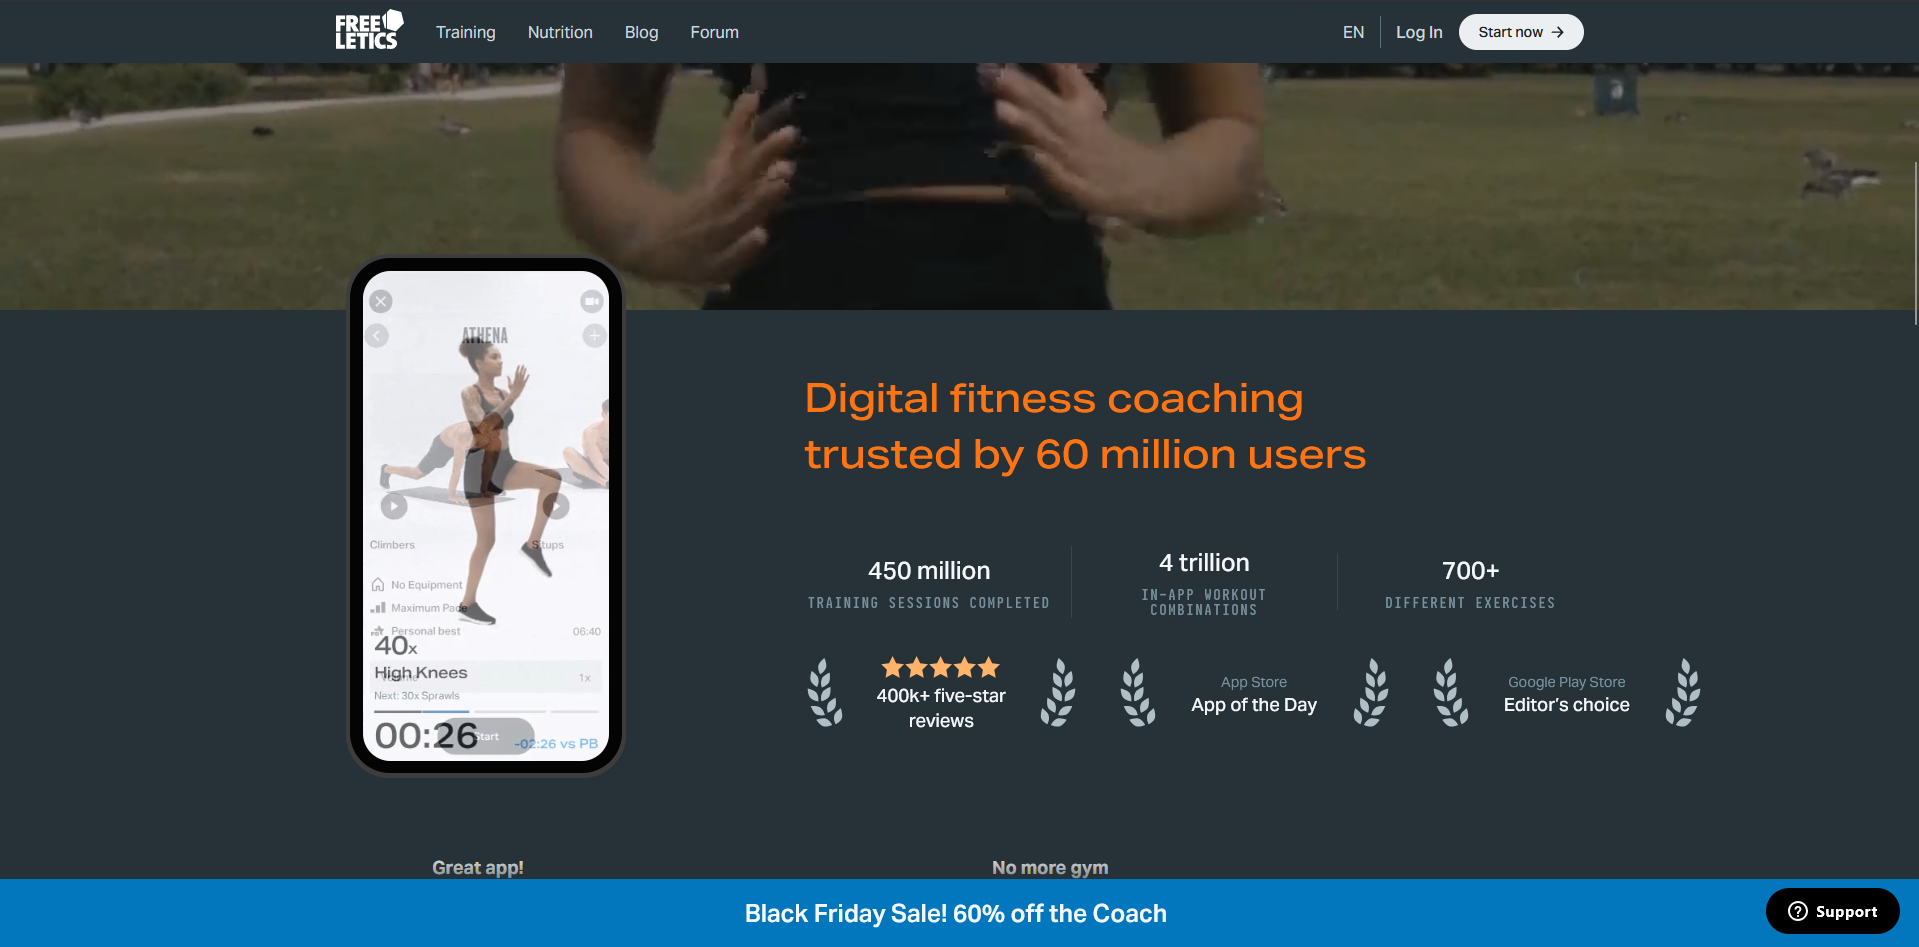
\includegraphics[width=0.85\textwidth]{freeletics.png}
  \caption{Spletna stran Freeletics s ponudbo paketov \cite{freeletics_web}.}
  \label{fig:freeletics}
\end{figure}


\subsection{Garmin Connect+}

\paragraph{Opis.} Garmin Connect je brezplačna aplikacija in spletna stran za lastnike Garminovih ur. Marca 2025 je Garmin predstavil plačljivo nadgradnjo Connect+, ki stane 6,99~USD (8,99~EUR) na mesec ali 69,99~USD (89,99~EUR) na leto, vse obstoječe funkcije pa ostajajo brezplačne \cite{notebookcheck_garmin}.

\paragraph{Ključne funkcionalnosti.}
\begin{itemize}
  \item \emph{Active Intelligence} -- personalizirani nasveti na podlagi dnevnih podatkov \cite{androidheadlines_garmin};
  \item nadzorna plošča zmogljivosti s prilagodljivimi grafi \cite{androidheadlines_garmin};
  \item prikaz podatkov o vadbi v realnem času na telefonu;
  \item od januarja 2026 beleženje prehrane (podatkovna zbirka živil, skeniranje črtne kode, prepoznava hrane s kamero) \cite{androidauthority_garmin_nutri};
  \item brezplačni del: srčni utrip, spanje, stres, načrti treninga in spletni portal Garmin Connect.
\end{itemize}

\paragraph{Prednosti.} Zelo natančni podatki z ure, obsežen brezplačni del, sorazmerno nizka cena naročnine.

\paragraph{Slabosti.} Namenjen le lastnikom Garminovih naprav, vmesnik je zaradi količine podatkov za začetnike zahteven, uvedba plačljivega dela je naletela na negativen odziv uporabnikov \cite{tomsguide_garmin}.

\begin{figure}[H]
  \centering
  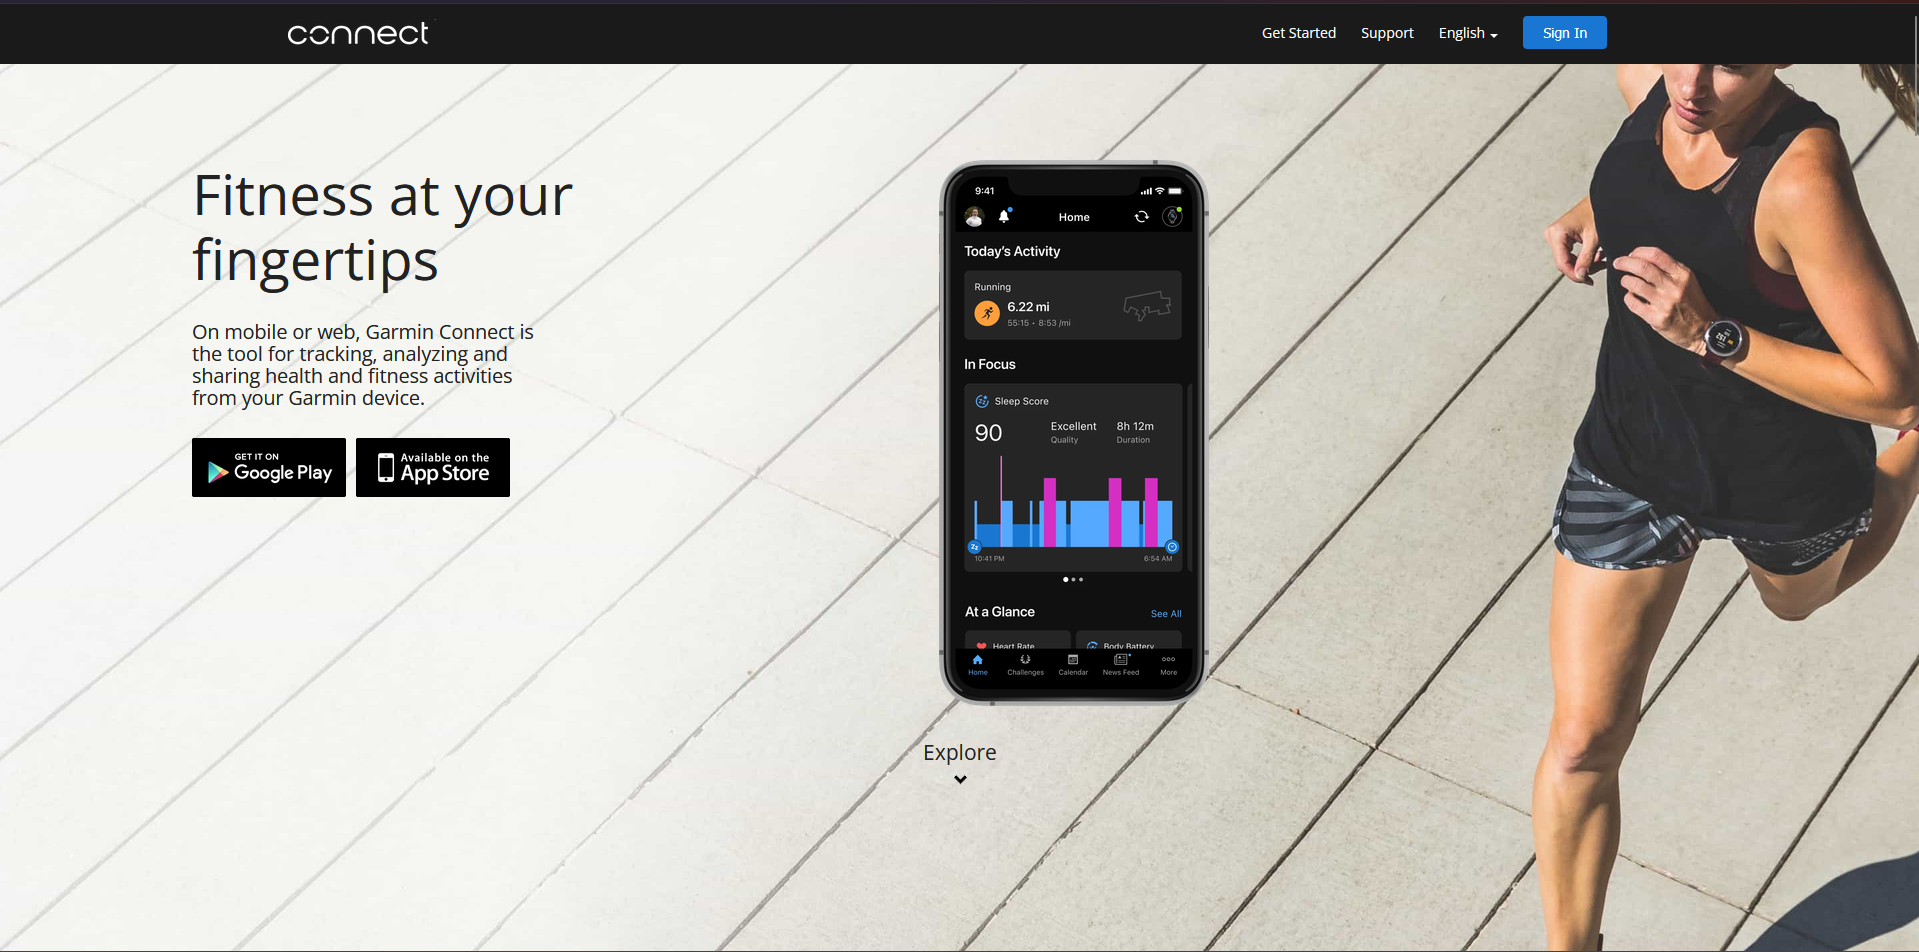
\includegraphics[width=0.85\textwidth]{garmin_connect.png}
  \caption{Spletni portal Garmin Connect \cite{garmin_web}.}
  \label{fig:garmin}
\end{figure}

\subsection{Primerjava}

\begin{table}[H]
  \centering
  \small\setlength{\tabcolsep}{4pt}
  \begin{tabular}{lcccc}
    \toprule
    & \textbf{Google Health} & \textbf{Strava} & \textbf{Freeletics} & \textbf{Garmin Connect+} \\
    \midrule
    Brezplačna različica      & da & da & omejena & da \\
    Načrti vadbe za različne cilje & da & delno & da & delno \\
    Beleženje prehrane         & da & ne & ločena aplikacija & da (plačljivo) \\
    Neodvisnost od naprave     & ne & da & da & ne \\
    Cenik na spletni strani    & da & da & da & da \\
    Slovenski jezik            & ne & ne & ne & ne \\
    \bottomrule
  \end{tabular}
  \caption{Primerjava pregledanih rešitev.}
  \label{tab:primerjava}
\end{table}

\section{Zaključek}

\paragraph{Kaj bomo prevzeli.} Od vseh pregledanih rešitev bomo na spletni strani prevzeli jasno predstavitev modela \emph{brezplačna osnova + plačljivi paketi} s preglednim cenikom (po zgledu Freeletics in Garmina). Od Freeletics bomo prevzeli predstavitev načrtov vadbe glede na cilj uporabnika, od Google Health in Garmina pa predstavitev funkcionalnosti s posnetki zaslona aplikacije in kratkimi opisi. Od Strave bomo prevzeli poudarek na motivaciji in izzivih, ki jih bomo izpostavili že na domači strani.

\paragraph{Kaj bo SloFit naredil drugače ali bolje.}
\begin{itemize}
  \item \textbf{Slovenski jezik in lokalni trg} -- nobena od pregledanih rešitev ni v slovenščini; spletna stran in aplikacija bosta v celoti slovenski, s cenami v evrih in podjetjem s sedežem v Mariboru.
  \item \textbf{Vse na enem mestu} -- vadba, beleženje treningov, prehrana in izzivi v eni aplikaciji, medtem ko ima Freeletics prehrano v ločeni aplikaciji, Strava pa je ne ponuja.
  \item \textbf{Neodvisnost od naprave} -- za razliko od Google Health in Garmina SloFit za uporabo ne zahteva nakupa določene pametne ure.
  \item \textbf{Za začetnike in izkušene} -- preprosta predstavitev na spletni strani in pripravljeni načrti vadbe, brez zahtevnega vmesnika, ki ga ima npr. Garmin.
  \item \textbf{Pregledne cene in hiter prenos} -- vsi paketi bodo jasno prikazani na eni strani, prenos aplikacije (App Store, Google Play, QR koda) in kontakt s podjetjem pa bosta dostopna z vsake podstrani.
\end{itemize}

\sloppy
\begin{thebibliography}{99}

\bibitem{freedom251} Is Fitbit Premium Worth the \$9.99 Monthly Cost? Dostopno na: \url{https://freedom251.com/is-fitbit-premium-worth-the-9-99-monthly-cost/} [24.~11.~2026].

\bibitem{androidauthority_gh} Android Authority: Google Health Premium price, inclusions and features. Dostopno na: \url{https://androidauthority.com/google-health-premium-price-inclusions-features-3664507/} [24.~11.~2026].

\bibitem{googlestore_fitbit} Google Store: Google Health Premium. Dostopno na: \url{https://store.google.com/product/fitbit_premium} [24.~11.~2026].

\bibitem{wareable_fitbit} Wareable: What is Fitbit Premium and is it worth it? Dostopno na: \url{https://www.wareable.com/fitbit/guide-to-fitbit-premium-8162} [24.~11.~2026].

\bibitem{techradar_fitbit} TechRadar: Fitbit Premium review. Dostopno na: \url{https://www.techradar.com/health-fitness/fitbit-premium-review} [24.~11.~2026].

\bibitem{wareable_strava} Wareable: Is Strava membership worth it? Dostopno na: \url{https://www.wareable.com/sport/is-strava-premium-worth-it} [24.~11.~2026].

\bibitem{bikeradar_strava} BikeRadar: Strava hikes monthly subscription price. Dostopno na: \url{https://www.bikeradar.com/news/strava-hikes-monthly-subscription-cost-by-more-than-25-per-cent/} [24.~11.~2026].

\bibitem{techradar_strava} TechRadar: Strava review. Dostopno na: \url{https://www.techradar.com/health-fitness/strava-is-still-the-best-training-app-for-runners-and-cyclists-but-its-getting-expensive} [24.~11.~2026].

\bibitem{strava_web} Strava. Dostopno na: \url{https://www.strava.com} [24.~11.~2026].

\bibitem{freeletics_appstore} Freeletics: Workouts \& Fitness, App Store. Dostopno na: \url{https://apps.apple.com/app/id654810212} [24.~11.~2026].

\bibitem{freeletics_help} Freeletics Help Center: Purchase a Coach subscription. Dostopno na: \url{https://help.freeletics.com/hc/en-us/articles/360020109819-Purchase-a-Coach-subscription} [24.~11.~2026].

\bibitem{ggr_freeletics} Garage Gym Reviews: Freeletics. Dostopno na: \url{https://www.garagegymreviews.com/?p=170520} [24.~11.~2026].

\bibitem{paddle_freeletics} Paddle: Does Freeletics' Pricing Strategy Need to Hit the Gym? Dostopno na: \url{https://www.paddle.com/studios/shows/pricing-page-teardown/does-freeletics-pricing-strategy-need-to-hit-the-gym} [24.~11.~2026].

\bibitem{freeletics_web} Freeletics. Dostopno na: \url{https://www.freeletics.com} [24.~11.~2026].

\bibitem{notebookcheck_garmin} Notebookcheck: Garmin Connect+ -- new subscriber-only features. Dostopno na: \url{https://www.notebookcheck.net/Garmin-Connect-New-subscriber-only-features-arrive-for-smartwatch-users.988232.0.html} [24.~11.~2026].

\bibitem{androidheadlines_garmin} Android Headlines: Garmin Connect Plus paid subscription. Dostopno na: \url{https://www.androidheadlines.com/2025/03/garmin-connect-plus-paid-subscription.html} [24.~11.~2026].

\bibitem{tomsguide_garmin} Tom's Guide: Garmin sparks outrage with Connect+ subscription paywall. Dostopno na: \url{https://www.tomsguide.com/wellness/smartwatches/garmin-sparks-outrage-with-connect-subscription-paywall-have-your-say} [24.~11.~2026].

\bibitem{androidauthority_garmin_nutri} Android Authority: Garmin finally adds native food tracking. Dostopno na: \url{https://www.androidauthority.com/garmin-connect-nutrition-tracking-feature-3629846} [24.~11.~2026].

\bibitem{garmin_web} Garmin Connect. Dostopno na: \url{https://connect.garmin.com} [24.~11.~2026].

\end{thebibliography}

\end{document}
